\chapter{Virtualizzazione}
\label{chap:virt}

Quanto descritto nel capitolo precedente costituisce il livello più alto dell'architettura NFV, le \textit{Virtualized Network Functions} (VNFs). In particolare, si descrive il software in grado di svolgere una determinata funzione virtuale: il router. Queste pagine invece si pongono l'obiettivo di fornire una panoramica in cui inquadrare lo strato infrastrutturale, presentando alcune tecnologie fondazionali di virtualizzazione e tratteggiando il ruolo dell'orchestratore.

\section{SR-IOV}

Parlando di DPDK si è dato per scontato che una scheda di rete potesse essere assegnata ad una VNF senza problemi e senza overhead. In effetti i moderni hypervisor consentono di destinare un intero device ad una macchina virtuale o ad un container, nel primo caso con un'operazione detta ``PCI Passthrough'', nel secondo spostando il dispositivo nel namespace desiderato. Cosa succede però se una stessa interfaccia deve essere assegnata a più entità, scenario comune nelle architetture complesse? La soluzione solitamente consiste nel creare un bridge, ossia uno switch virtuale in kernel che emuli più NIC virtuali sopra una sola fisica, vanificando però le ottimizzazioni in capo a DPDK.

\begin{figure}[htb]
    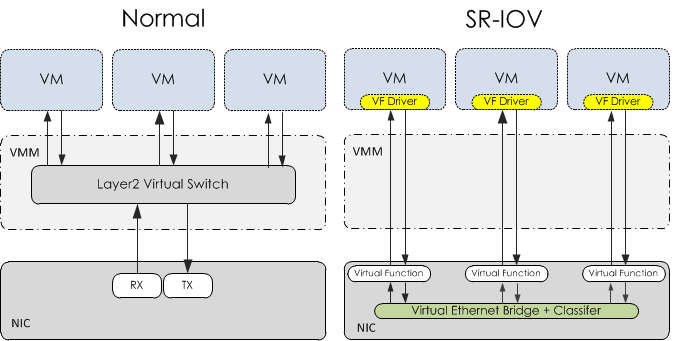
\includegraphics[width=0.7\textwidth]{graphics/sriov_overview.png}
    \caption{Bridge virtuale vs SR-IOV}
    \label{fig:sriov-overview}
\end{figure}

Single Root I/O Virtualization (SR-IOV) è una funzionalità di PCI Express Extended che permette ad un dispositivo fisico di apparire come più dispositivi virtuali. Il dispositivo fisico è denominato \textit{Physical Function} (PF) mentre i dispositivi virtuali sono chiamati \textit{Virtual Functions} (VF). Grazie a SR-IOV è possibile accedere a ciascuna funzione virtuale tramite un indirizzo PCIe univoco. Ogni device virtuale ha il proprio spazio di memoria PCI, che viene utilizzato per mappare il suo set di registri ed il driver del dispositivo virtuale opera su di essi al pari di uno fisico, mascherando l'astrazione al sistema operativo.

Nel caso delle schede di rete, ogni interfaccia è dotata di un proprio indirizzo di livello 2 (MAC) e di buffer in ricezione ed invio dedicati. Il bridging prima effettuato dal kernel viene adesso svolto dal microcontrollore a bordo della scheda di rete. Una NIC che supporti DPDK ed SR-IOV è dunque in grado di essere assegnata contemporaneamente a più VNFs senza comprometterne le performance ed in maniera trasparente.

Spostare lo switch virtuale verso il dispositivo fisico ha però lo svantaggio di allungare il percorso quando i pacchetti sono destinati ad una VNF sullo stesso server di quella mittente, occupando il bus PCI inutilmente. Alcuni studi recenti aprono alla possibilità di realizzare uno switch virtuale con DPDK (OVS-DPDK) e ipotizzano diverse tipologie di traffico: est-ovest per la comunicazione tra VNF nello stesso dominio, nord-sud altrimenti. I risultati dipendono molto dalla natura del traffico e non emerge un chiaro vincitore: uno switch virtuale basato su DPDK è preferibile in caso di pattern est-ovest, ma bisogna prestare attenzione al tipo di funzione che si vuole realizzare e se questa possa o meno trarre beneficio dall'uso di un approccio vettoriale come VPP. In tutti gli altri casi, si dimostra come SR-IOV scali linearmente all'aumentare di funzioni virtuali \cite{intel-sriov, cisco-sriov}.

\section{KVM}

Risalendo lo stack infrastrutturale, appena sopra l'hardware, troviamo il layer di virtualizzazione. Lo scopo di questo livello intermedio è quello di astrarre, partizionare e gestire le risorse fisiche del server potendone permettere l'assegnazione a più funzioni virtuali. Non si parla ancora di gestione federata, per adesso il focus è incentrato sul singolo host.

\textit{Kernel-based Virtual Machine} (KVM) è un modulo di Linux che trasforma il kernel in un hypervisor, rendendolo in grado di ospitare ed eseguire macchine virtuali, assegnando risorse come numero di core, quantità di memoria RAM e dispositivi fisici. In KVM, ogni CPU virtuale è mappata su un thread del sistema operativo, operazione necessaria a garantirne il corretto isolamento. Sopra i processori così realizzati viene eseguito il sistema operativo guest proprio della macchina virtuale e tutte le relative applicazioni.

\begin{figure}[htb]
    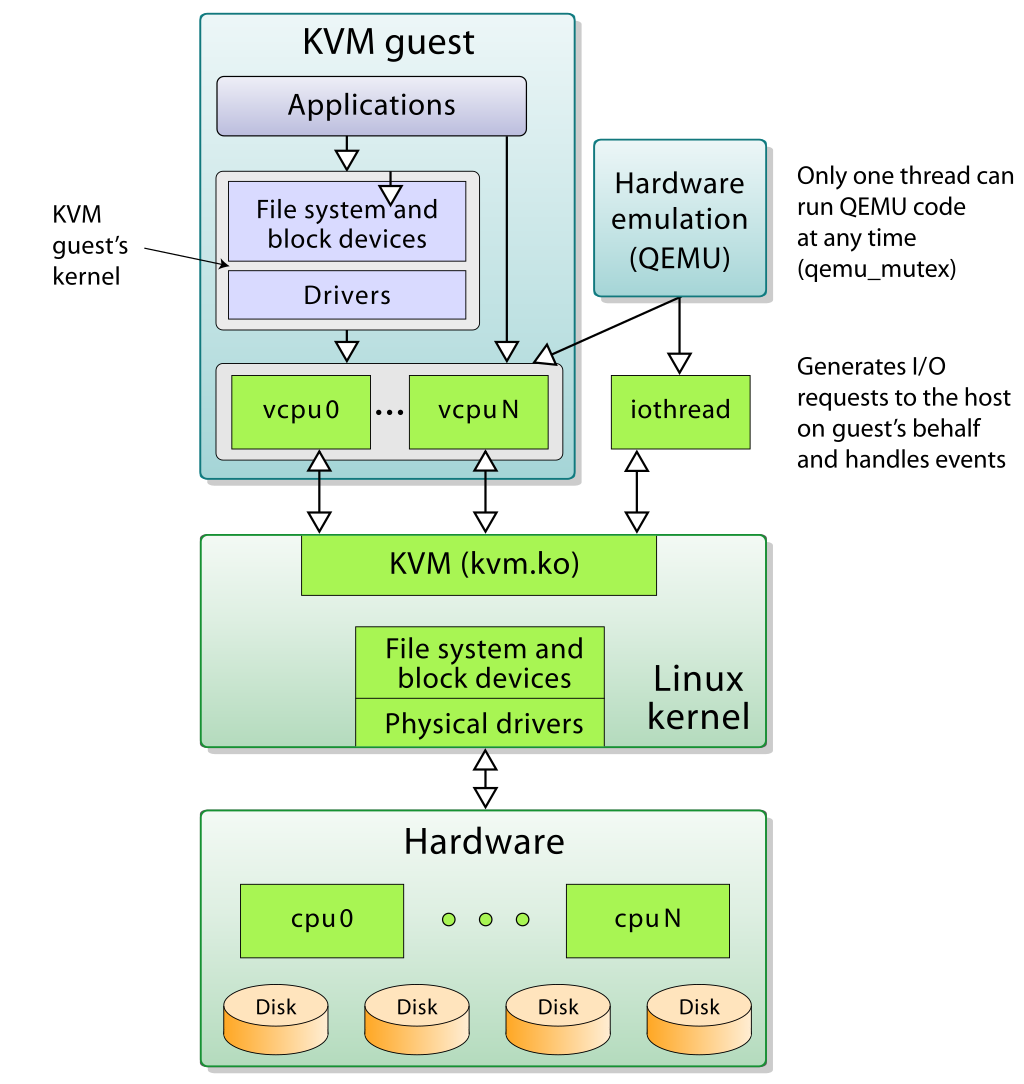
\includegraphics[width=0.7\textwidth]{graphics/kvm.png}
    \caption{Architettura di KVM}
    \label{fig:kvm-arch}
\end{figure}

Nello schema proposto in \cref{fig:sriov-overview} KVM è rappresentato dal \eng{Virtual Machine Monitor} (VMM) ed ha il compito di assegnare funzioni virtuali della NIC SR-IOV alle diverse VM, dando loro diretto accesso al bus PCI. Non è genericamente compito dell'hypervisor emulare dispositivi virtuali, motivo per cui KVM è spesso usato in accoppiata con un altro software: QEMU. Emulare un device via software ne riduce le performance e per questo si cerca di limitarne gli usi a quelle periferiche ``lente'' necessarie al corretto funzionamento delle macchine virtuali come mouse, tastiera e uscita video.

\section{NUMA}

I sistemi multi-CPU sono una realtà consolidata. La domanda di potenza computazionale cresce molto più rapidamente della capacità dei processori, inevitabilmente limitati dalla legge di Moore. Le architetture multicore sono complesse da progettare e la loro scalabilità limitata: mettere troppi core su un singolo chip non è possibile perché il segnale di clock impiegherebbe troppo tempo per propagarsi. Inoltre, il calore generato sarebbe eccessivo e i continui messaggi di aggiornamento delle cache condivise finirebbero col saturare la trama di interconnessione ed i core stessi.

L'alternativa è rappresentata dai sistemi multi-processore in cui più CPU identiche trovano spazio sulla medesima scheda madre e sono collegate da dei bus. L'organizzazione può essere di due tipi:

\begin{itemize}
    \item Tutti i processori vedono tutta la memoria indiscriminatamente e per questo vengono chiamati sistemi \textit{Uniform Memory Access} (UMA)
    \item Ciascuna CPU è direttamente connessa ad una porzione di memoria e può accedere al resto tramite le altre CPU, \textit{Non-Uniform Memory Access} (NUMA)
\end{itemize}

Le architetture UMA sono naturalmente le più semplici da progettare e da gestire, ma non sono le più efficienti. La memoria rischia di saturarsi velocemente sotto il carico di decine di core che eseguono operazioni di lettura e scrittura contemporaneamente, ponendo un serio limite alla scalabilità del sistema. Viceversa NUMA consente di sfruttare il principio di località dei dati e dei programmi, ridistribuendo il carico per aree. Lo svantaggio è che il sistema operativo ed il progettista devono tener conto del layout sottostante ed elaborare soluzioni ``NUMA-aware'' che ripartiscano il lavoro tra i processori e le memorie sulla base dei dati acceduti più frequentemente.

\begin{figure}[htb]
    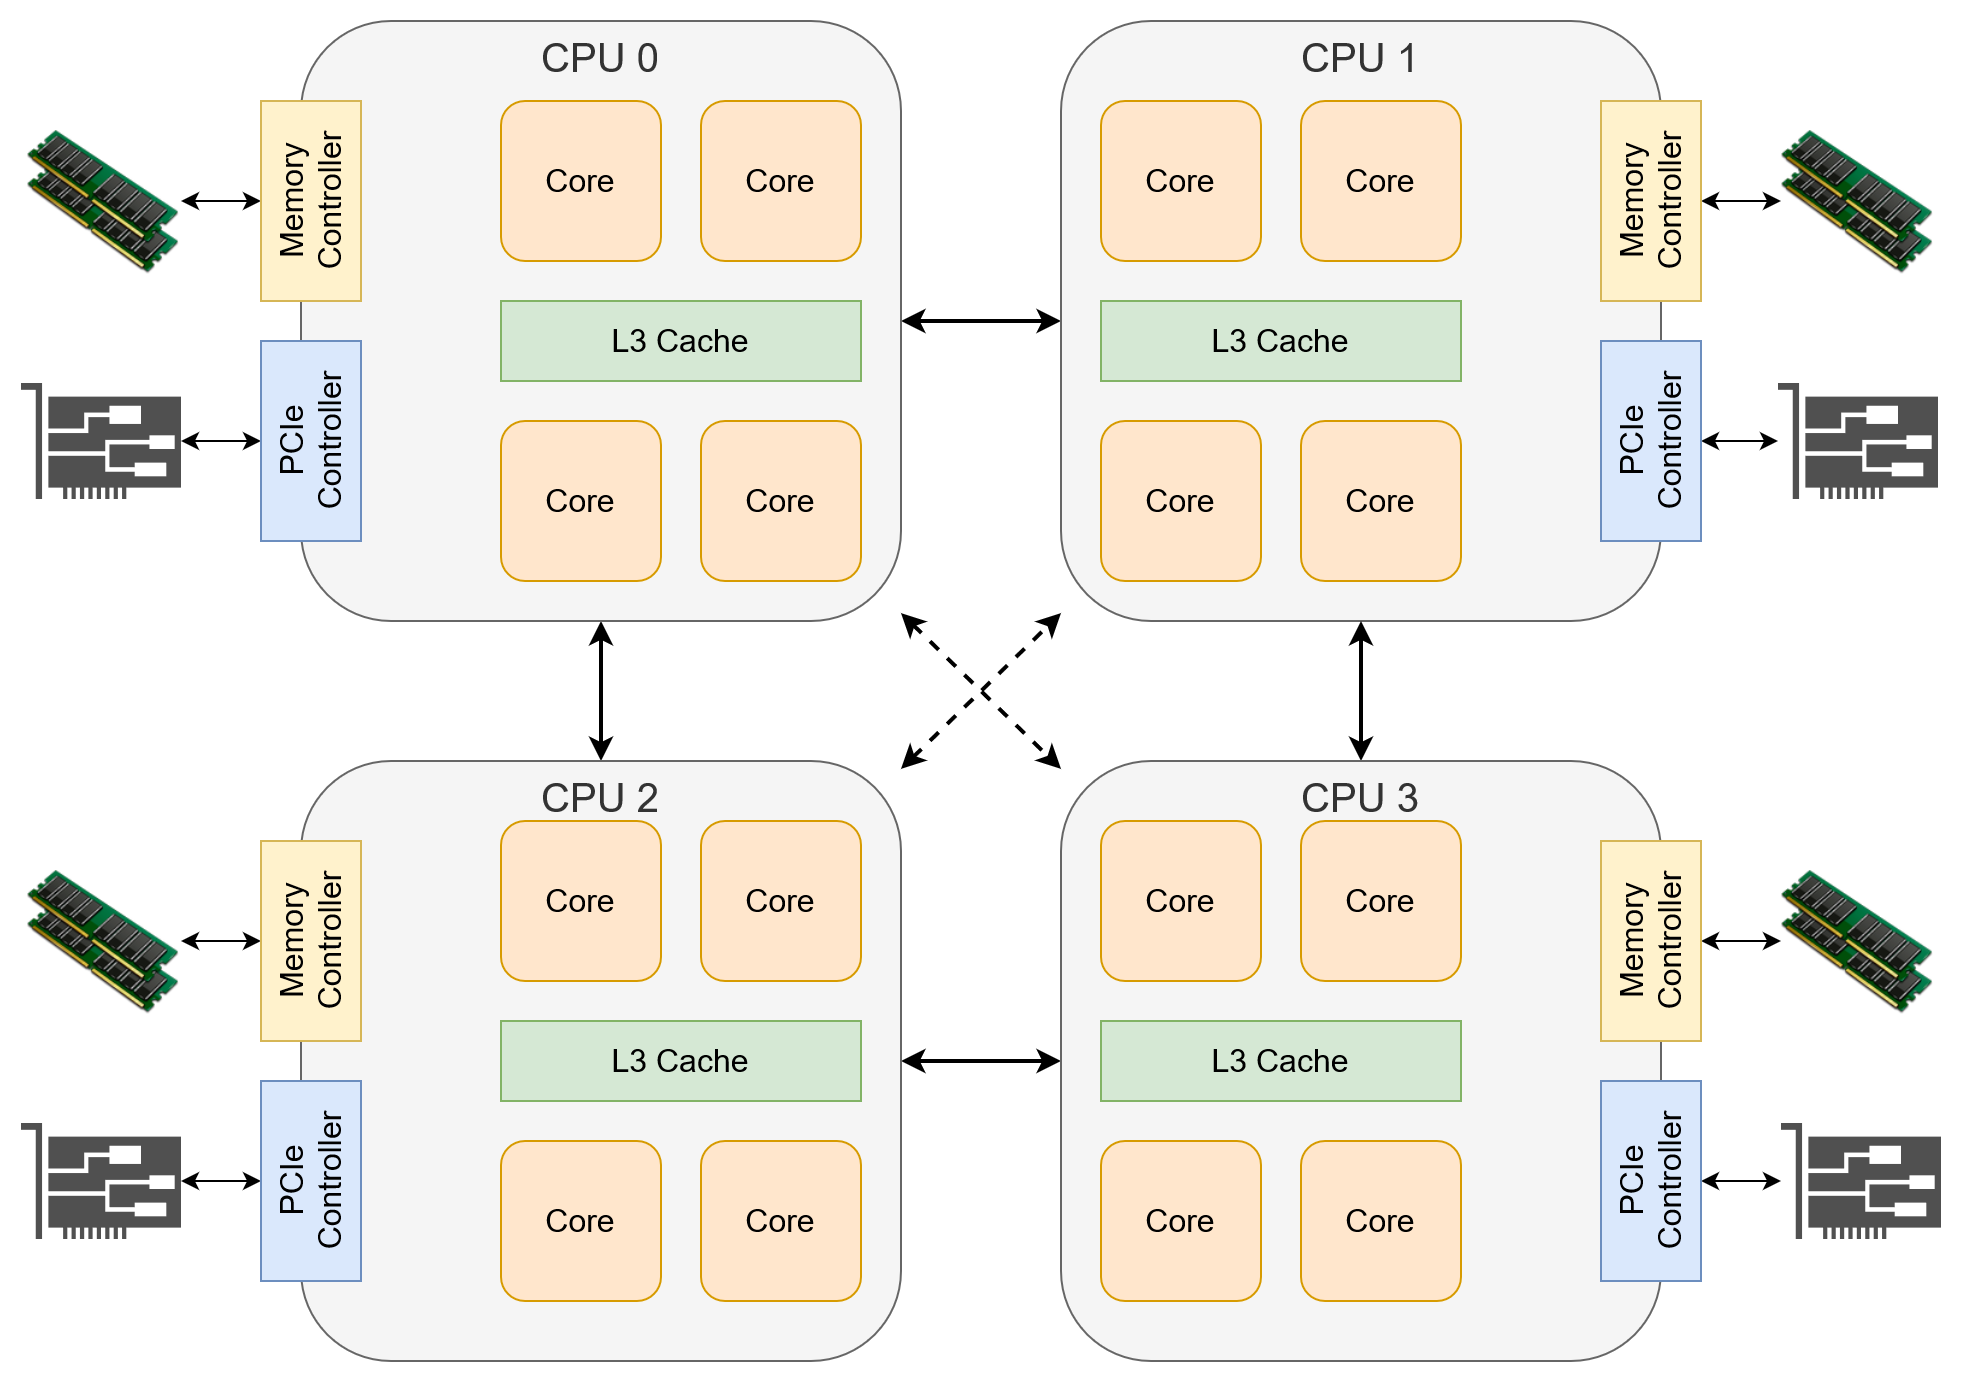
\includegraphics[width=0.8\textwidth]{graphics/numa.png}
    \caption{Layout NUMA}
    \label{fig:numa}
\end{figure}

Ciascun insieme di CPU, memoria e dispositivi direttamente connessi tra loro costituisce un ``nodo NUMA''. I nodi NUMA possono essere interconnessi in vari modi: singolo bus condiviso, anello, maglia completa,... in funzione delle potenzialità richieste e del prezzo. Per stimare il costo di passare da un nodo ad un altro, Linux usa una matrice delle distanze, una sorta di grafo che rappresenta la latenza nell'accedere ad una porzione di memoria: accedere alla propria memoria ha un valore di default pari a 10 mentre quello degli altri nodi dipende dal layout fisico.

Non solo la memoria, ma anche i dispositivi sono da tenere in considerazione: una scheda di rete direttamente connessa ad una CPU potrà minimizzare le latenze e massimizzare il throughput solo se il software con cui dialoga è fisicamente situato sullo stesso processore. Diversamente i dati dovranno attraversare la fabric di interconnessione cosa che nel complesso potrebbe avere ripercussioni pesanti su tutto il sistema.

Come discusso nel \cref{chap:lab}, un'allocazione ragionata delle VNFs che tenga conto della topologia sottostante può avere importanti benefici sulle performance, soprattutto in condizioni di elevato carico del server. Il progettista deve porre la dovuta attenzione nella definizione dei requisiti della VNF alla luce dei software che essa ospita e l'orchestratore dev'essere in grado di allocare le risorse di conseguenza.

\begin{figure}[htb]%
    \centering
    \subfloat[Accesso remoto]{{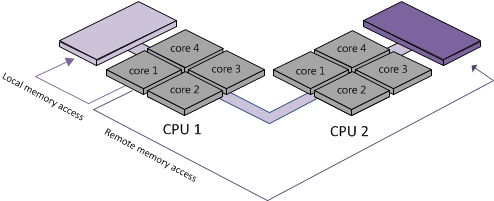
\includegraphics[width=0.45\textwidth]{graphics/numa-vm-1.png} }}%
    \qquad
    \subfloat[Pinning delle risorse]{{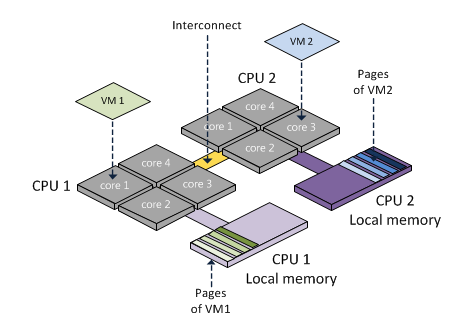
\includegraphics[width=0.45\textwidth]{graphics/numa-vm-2.png} }}%
    \caption{Esempi di allocazione NUMA-aware}%
    \label{fig:example}%
\end{figure}

\section{OpenStack}

Il paragrafo precedente descrive il ruolo del layer di virtualizzazione, centrale nella realizzazione dell'infrastruttura NFV (NFVI, \cref{fig:esti-nfv-low-level}). È bene ricordare che KVM non è l'unica possibile alternativa: come detto il framework ETSI NFV è agnostico rispetto alla tecnologia. Un hypervisor fine a se stesso però non è molto utile, serve un'infrastruttura in grado di gestire automaticamente centinaia se non migliaia di server con ancor più macchine virtuali e container.

Nell'ultimo decennio l'industria ha fatto passi da gigante in questa direzione, producendo gli \textit{orchestratori}, software in grado di far incontrare la disponibilità fisica di risorse con la domanda dei servizi, incastrando requisiti e funzionalità e fornendo altresì delle metriche relative all'esecuzione. In quest'ottica s'inserisce OpenStack, una piattaforma di cloud computing aperta e multi-vendor tra le più usate al mondo. Composto da una miriade di sotto-progetti che spaziano dal compute allo storage passando per load balancer, billing e monitoring, OpenStack è perfetto per assolvere le funzioni di NFVI e VIM (Virtualized Infrastructure Manager).

Tra i progetti di cui si compone, vi è Tacker, un modulo che implementa la parte alta di NFV MANO (VNF Manager e NFV Orchestrator) facendosi carico del ciclo vitale delle istanze VNF. La natura aperta di OpenStack lo rende facilmente interoperabile con altre soluzioni, tanto che chi non volesse usare Tacker può avvalersi di Open Source MANO per il macro-blocco di management e orchestration il quale dialoga con il livello infrastrutturale di OpenStack tramite la Northbound API.

\begin{figure}[htb]
    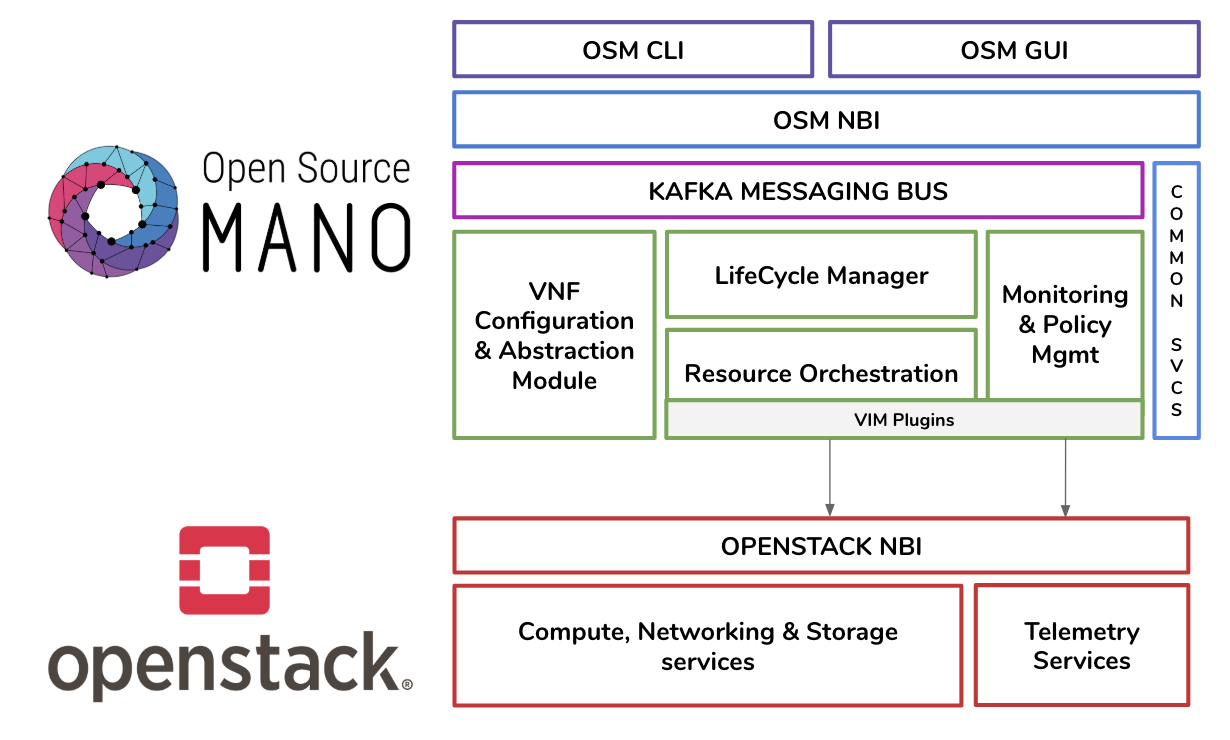
\includegraphics[width=0.7\textwidth]{graphics/openstack-mano.png}
    \caption{Northbound API tra OpenStack e Open Source MANO}
    \label{fig:openstack-mano}
\end{figure}

Vale la pena notare che ciascuno dei componenti qua citati è in realtà un software completo, costituito da vari servizi che segue un iter di sviluppo proprio. La complessità di tutte queste ``parti mobili'' ed il modo in cui esse interagiscono tra loro tramite API standard ricorda quella di un sistema operativo, tant'è che s'inizia a parlare di \textit{cloud operating system} o \textit{network operating system}.

% Tacker is an official OpenStack project building a Generic VNF Manager (VNFM) and an NFV Orchestrator (NFVO) to deploy and operate Network Services and Virtual Network Functions (VNFs) on an NFV infrastructure platform like OpenStack. It is based on ETSI MANO Architectural Framework and provides a functional stack to Orchestrate Network Services end-to-end using VNFs.

\section{VMware vCloud NFV}

La possibilità di realizzare un'architettura vasta come ETSI NFV da zero, monetizzando sui prodotti, ha attirato l'attenzione di nuovi vendor, intenti a proporre le loro soluzioni frutto di decenni di esperienza nell'ambito del cloud. Tra questi, è sicuramente degna di nota VMware, azienda leader nel settore della virtualizzazione che ha creato una famiglia di prodotti integrati per implementare i componenti NFVI e MANO di NFV.

La soluzione è proprietaria ed è la seconda più utilizzata dai grandi operatori che preferiscono appoggiarsi su aziende affermate per poter garantire la continuità di business. Né OpenStack né VMware però si occupano della parte VNF: quella richiede specifiche conoscenze di networking e protocolli e spesso ricade sui vecchi player del mercato. Ad esempio Cisco produce il sistema operativo IOS XRv che ricalca quello presente sulle moderne appliance fisiche dell'azienda e lo stesso fa Juniper con vMX. Nel segmento mobile Nokia ed Ericsson rappresentano due importanti player europei attivi nello sviluppo di gateway ed altri elementi virtuali facenti parte del panorama LTE e 5G.

\begin{figure}[htb]
    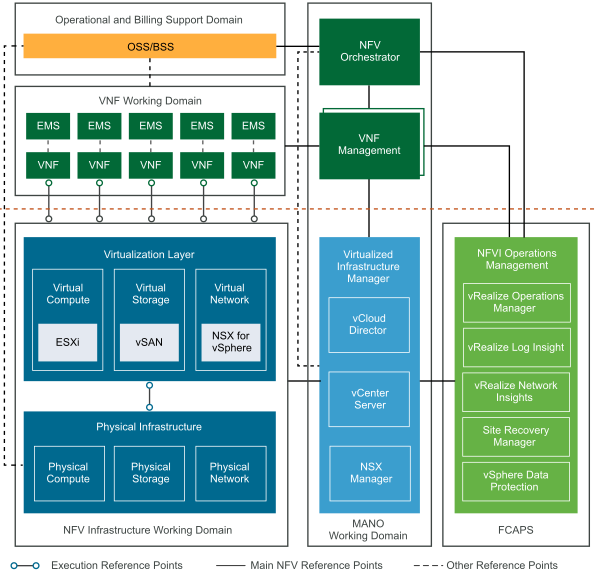
\includegraphics[width=0.7\textwidth]{graphics/vmware-nfv.png}
    \caption{Mapping dei prodotti VMware sull'architettura NFV \cite{vmware-vcloud}}
    \label{fig:vmware-nfv}
\end{figure}

% https://images.app.goo.gl/N55na3PmGGpkuGDd6
% \cite{vmware-vcloud} % https://images.app.goo.gl/3xsvPs54523TKozu9

% Ovviamente pure RedHat c'ha la sua, ne vogliamo parlare?
% https://images.app.goo.gl/gJxkHNwEEjgpzrx18